In this chapter we describe a software framework called Rheos, which demonstrates an approach for reasoning about large genomic datasets utilizing concepts of service-orientation and data streaming in contrast with traditional genomic data analysis frameworks\autocite{depristo2011framework} that take a procedural batch-based approach. Rheos' focus on service-orientation and streaming allow the users to make active tradeoff decisions between analysis time, cost, and quality as well as setting up precise operational Service Level Agreements, both between Rheos components, and between Rheos and external systems, as we describe in detail below.

\section{General Framework Design}

As already discussed in Chapters \ref{ch:introduction} and \ref{ch:background}, the general problem consists of collecting DNA samples from a population of individuals under study, sequencing these samples using Next Generation Sequencing techniques, identifying the mutations that are present, annotating their functional impact and utilizing the obtained data in a downstream data analysis with research or clinical decision-making goals. While there is a great variety of possible downstream analyses that may be performed depending on the individual goals of the analyst, there is a fairly well established set of steps for processing of the raw NGS data into a set of annotated variants, and it is these steps that we target with this work. The typical approach that is in widespread use today is to collect a batch of samples and then process each sample individually with a sequence of individual tools, that may be described via a higher-level workflow construct (such as in Figure \ref{fig:gatk_best_practices}, or using a framework like Butler, as described in Chapters \ref{ch:butler_architecture}, \ref{ch:butler_implementation}). There are, however, a number of factors that leave room for improvement in this model. These improvements lie along a set of dimensions that we describe briefly in the Introduction via a utility function $U_i = C_i + T_i + A_i$ for sample $i \in [1,N_s]$  that needs to be optimized, and that we describe in more detail here.

We use the following definitions throughout the text:

\begin{table}[!ht]
    \caption{Rheos common definitions}
    \label{tab:rheos_notation}
    {\begin{tabular}{lp{7cm}}
    \toprule
    Symbol & Description \\
    \midrule
    $N_p$ & Number of people \\
    $P = \{p_i : i \in [1,N_p]\}$ & Set of individuals under study \\
    $N_s$ & Number of samples \\
    $S = \{s_i : i \in [1,N_s]\}$ & Set of sequenced DNA samples. Each individual can have one or more samples. \\
    $A_i $ & Accuracy score of analysis for sample $i$ (precise definition of Accuracy TBD) \\
    $C_i = c_{g_i} + c_{s_i} + c_{a_i} + c_{r_i}$ & Cost score of data generation, storage, analysis, and retrieval respectively \\
    $T_i$ & Time score to process sample $i$ \\
    $U_i = C_i + T_i + A_i$ & A utility function for individual $i$ that penalizes high cost, high processing time, and low accuracy\\
    $U = \sum_{i=1}^{N_s} U_i$ & Overall utility of processing $N_s$ samples through Rheos.\\
    \bottomrule
    \end{tabular}}
\end{table}


\section{Data Streaming Architecture}

The overall technical architecture of the Rheos system is set up as a Service Oriented Architecture (SOA)\autocite{shaw1996software} which is an information system architecture paradigm where the overall problem that the system is trying to solve is broken down into a collection of loosely-coupled components called services. Each service has a well defined interface of inputs that it accepts and outputs that it produces. Services can be combined and orchestrated together to produce the overall desired output for the system. A key distinguishing feature of this architectural approach is that each service can be individually optimized to fulfill its contract most efficiently helping break down some of the performance limitations brought about by the necessity to simultaneously tackle competing constraints in more monolithic information system designs. Additionally, within a services framework, the dependencies between separate services can be negotiated not only in terms of service interfaces, but also in terms Service Level Agreements which constitute Quality of Service promises made by one service to its dependents\autocite{ingham2000constructing}. Because it is unlikely that a service designer will be able to accurately foresee all of the demands that will be placed on a service during its lifetime the SLAs provide a valuable feedback framework through which the service can be evaluated as it operates in production, as well as serving as a basis for negotiating evolving requirements between dependent services.

While general web services can support any data processing paradigm, in the Rheos framework we adopt a data streaming approach\autocite{babcock2002models}. In this approach we assume that the input to any service is a randomly ordered sequence of messages $M = {m_1, m_2, ....}$ where each message represents a fact about the underlying domain that the service reasons over, as well as some metadata, including an identifier, and a variety of timestamps of interest. The content of each message may provide a datum, such as the measurement of a quantity of interest, or signal that a particular event has taken place. It is in general assumed that the data stream is infinite in size, that messages may arrive out of order, and that any message that is placed in the stream is observed at most once, and may, in fact, never be observed. Messages are typically not sent directly from one service to another, instead the transfer of messages is mediated by a queuing system using a publish-subscribe\autocite{eugster2003many} model. Under this model each queue acts as a \emph{topic}. Message producers can publish data to the topic, and message consumers subscribe to receive messages from the topic. A message is consumed from the queue only after all of the subscribed consumers have seen it. End users retrieve information from the system via a set of User Interfaces that support both push (notifications) and pull (querying) models of data retrieval. A more detailed description of the architectural aspects of the system follows:

\subsection{Service-Oriented Data Streaming Model}

A data stream $M_{s,d} = {m_1, m_2, ....}$ is a sequence of datagrams transmitted over the network with the following properties:

\begin{itemize}
    \item The stream has a source $s$ and a destination $d$.
    \item A message $m$ in the stream is a tuple of the form $(header, payload)$, where:
    \begin{itemize}
        \item $header$ is a tuple of the form $(id, \dots)$ that holds at minimum a unique identifier $id$ for messages, and may hold additional metadata.
        \item $payload$ is an arbitrary data structure that holds the informational content of the message. 
    \end{itemize}
    \item $|M| = \infty$ by assumption.
    \item Messages may not arrive at destination $d$ in the same order that they were sent from source $s$.
    \item If $t_{i,s}$ is the time message $m_i$ leaves the source $s$ and $t_{i,d}$ is the time of arrival at destination $d$, then $\sup_i \{t_{i,d} - t_{i,s}\} = \infty$, i.e. a given sent message may never arrive at its destination.
\end{itemize}

A service $S = \{o_i\}$ is a collection of operations $o_i$ that act on one or more input data streams $\{M_i\}$ to produce one or more transformed output data streams $\{M_j\}$. Specifically:

An operation $O$ is a tuple of the form  $O = (i,o,p,f)$, where:
\begin{itemize} 
    \item $i = \{M_j, j \in [0, K]\}$ is a set of $K \ge 0$ input data streams.
    \item $o = \{M'_j, j \in [0, L]\}$ is a set of $L \ge 0$ output data streams.
    \item $f:M^K \mapsto M'^L$ is a transformation function that produces messages $m'$ in the output streams based on messages $m$ observed in the input streams.
    \item $p = \{p_i\}$ is a set of potentially optional query parameters.  
\end{itemize}

There are several distinct categories of operations that a service can perform on a set of input streams. We describe these here:

\paragraph{Windowing Function} - Service $S$ observes a sliding window, which is a sample of size $n$ of messages from stream $M_i$ and computes a summary statistic (see Figure \ref{fig:stream_window_function}) over the sample which is meant to be an approximation of the corresponding population parameter.

\begin{figure}[H]
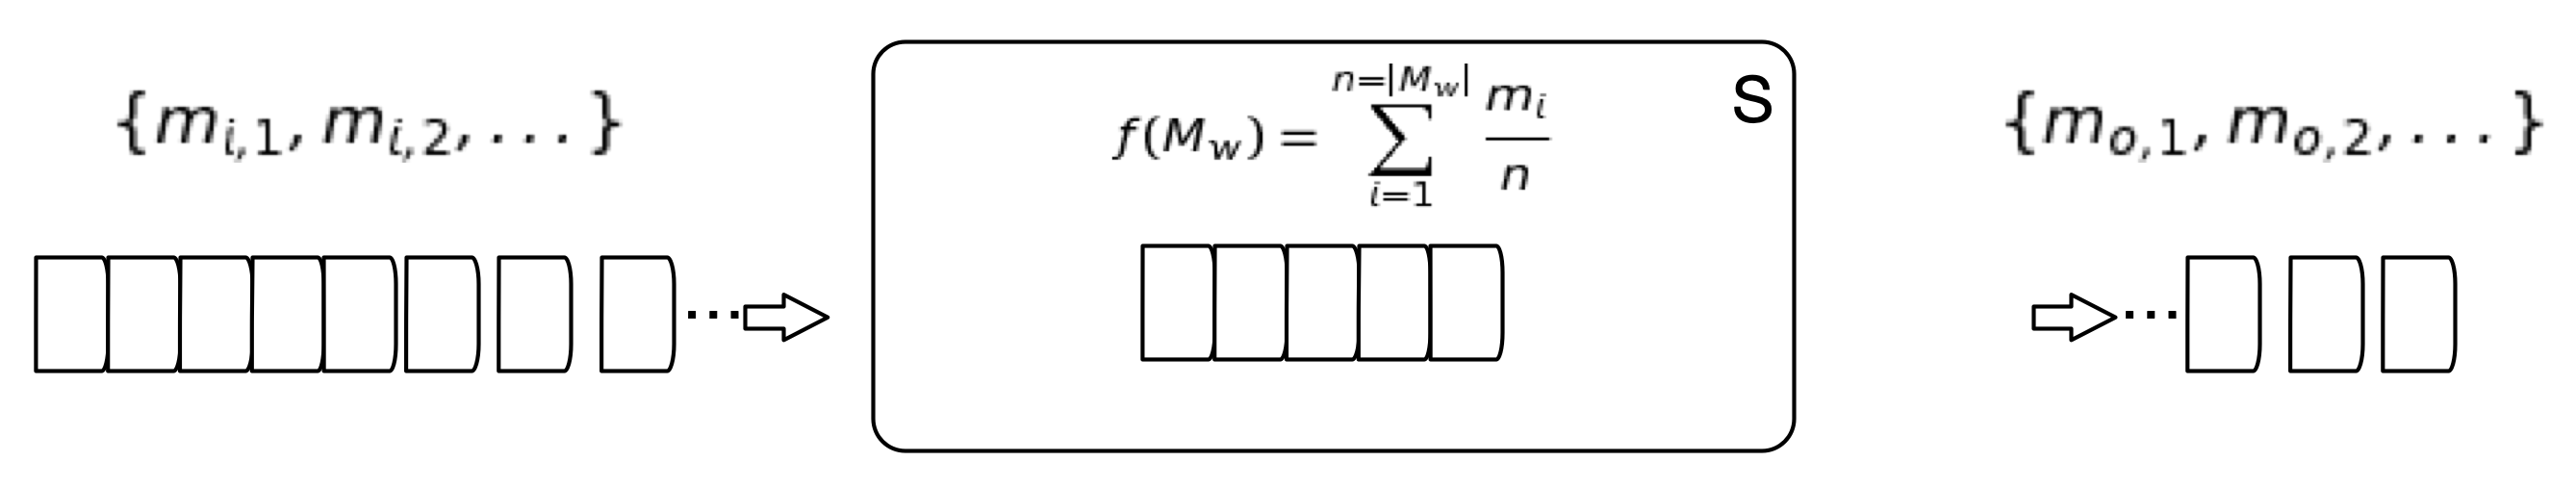
\includegraphics[scale=0.6]{stream_window_function}
\centering
\caption {Service S computes a summary statistic over a window of messages from stream $M$}
\label{fig:stream_window_function}
\end{figure}
 
\paragraph{Decorator Function} - Service $S$ observes messages $m_i$ and applies a function that augments (decorates) each message with additional attributes (see Figure \ref{fig:stream_decorator_function}) producing augmented messages $m_o$ as output.

\begin{figure}[H]
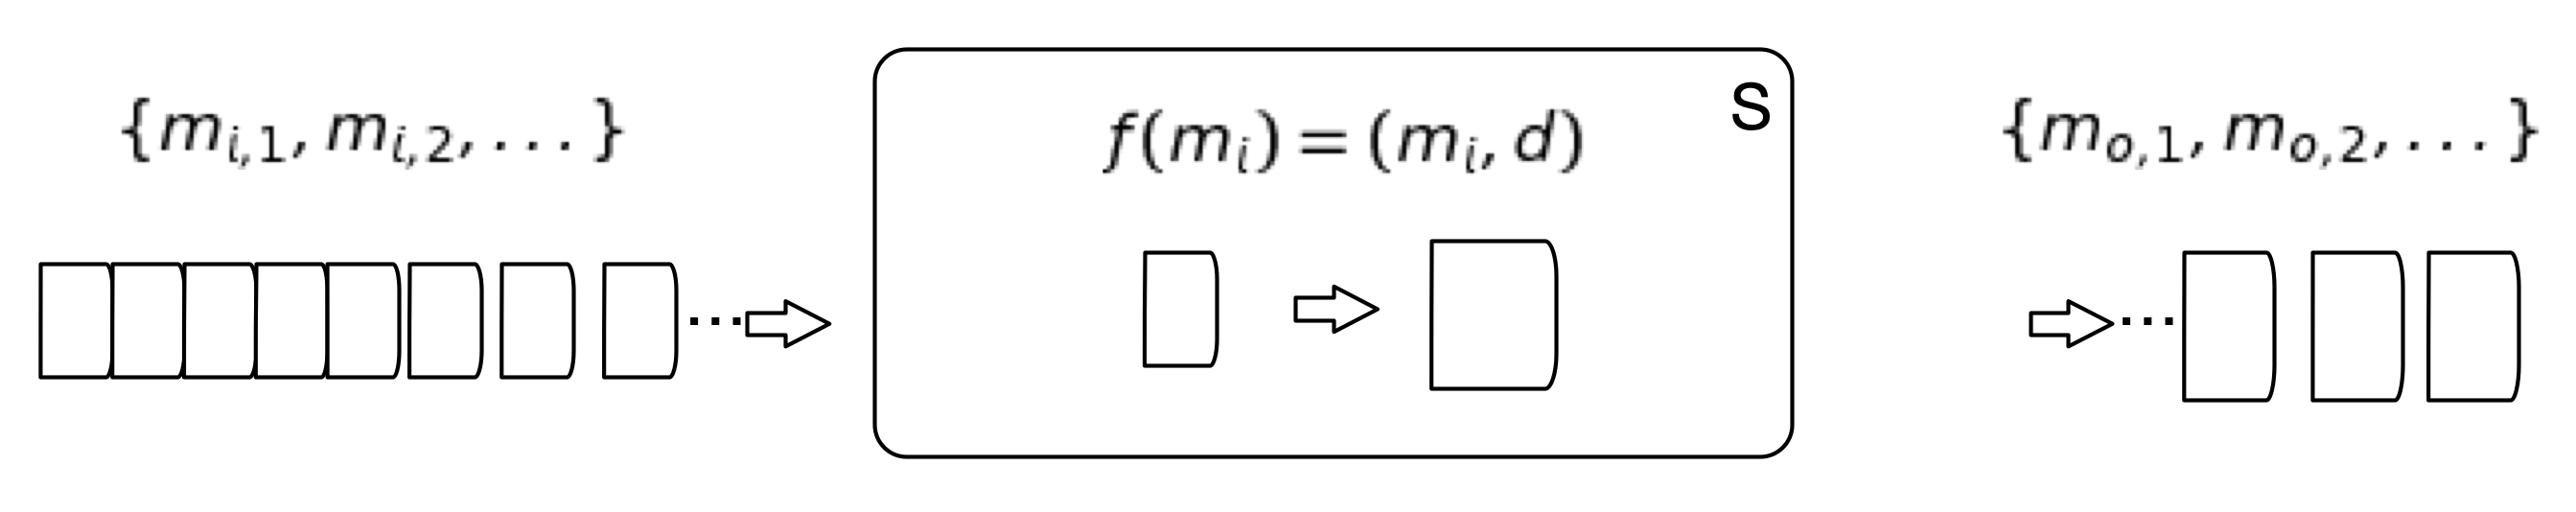
\includegraphics[scale=0.6]{stream_decorator_function}
\centering
\caption {Service S computes a summary statistic over a window of messages from stream $M$}
\label{fig:stream_decorator_function}
\end{figure}

\paragraph{Filter Function} - Service $S$ observes messages $m_i$ and applies a function $f:M\mapsto\{True,False\}$ that evaluates to a boolean value (see Figure \ref{fig:stream_decorator_function}). Only messages that map to $True$ are emitted as output.

\begin{figure}[H]
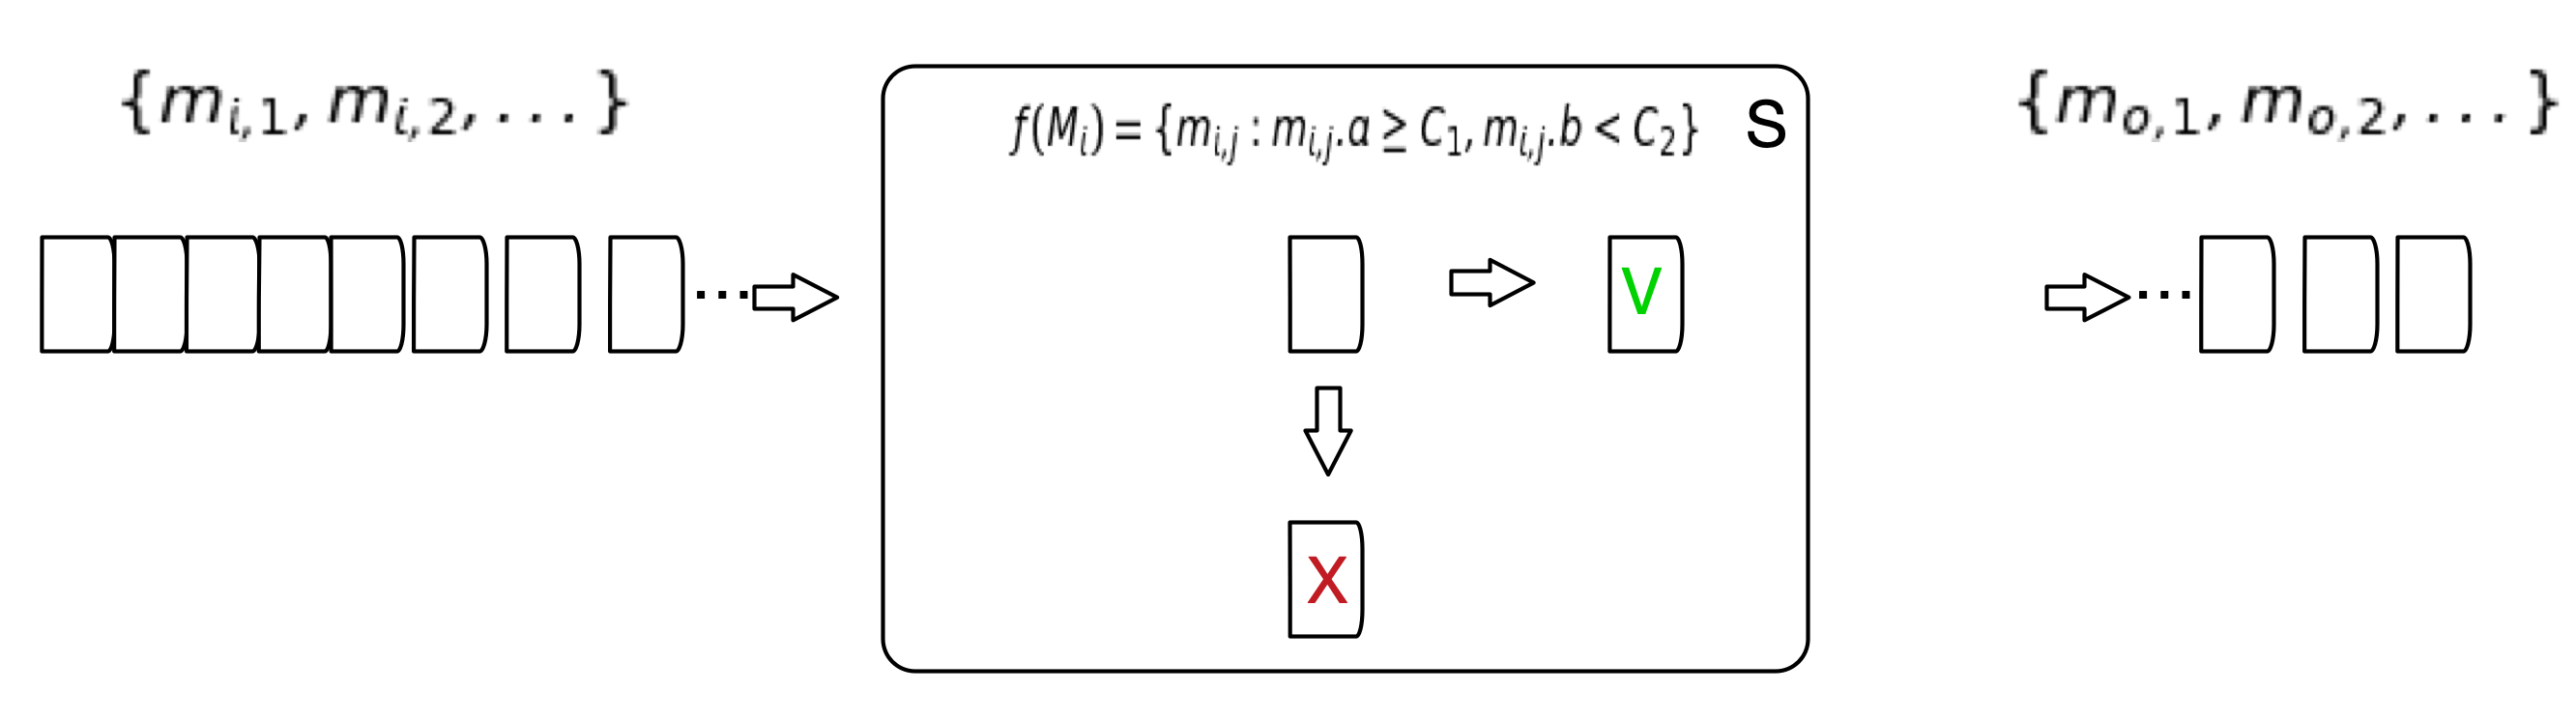
\includegraphics[scale=0.6]{stream_filter_function}
\centering
\caption {Service S filters messages from input stream $M$ and only allows through those that pass the filtering condition.}
\label{fig:stream_filter_function}
\end{figure}

\paragraph{Aggregator Function} - Service $S$ observes messages from $N$ different streams $\{M_j: j \in [1,N]\}$ and applies a function $f:M_i^N \mapsto M_o$ that aggregates messages from these streams to produce its output (see Figure \ref{fig:stream_aggregator_function}). Because aggregation happens over groups of messages that may not all arrive at the same time the service $S$ requires a mechanism for keeping local state so that it can accumulate messages that have already arrived while waiting for those that are necessary to compute $f$ yet have not been observed. The statefulness requirement of this type of service places an extra level of complexity (related to state-management and request routing) as well as inherent scalability limitations compared to stateless services\autocite{oppenheimer2002architecture}.

\begin{figure}[H]
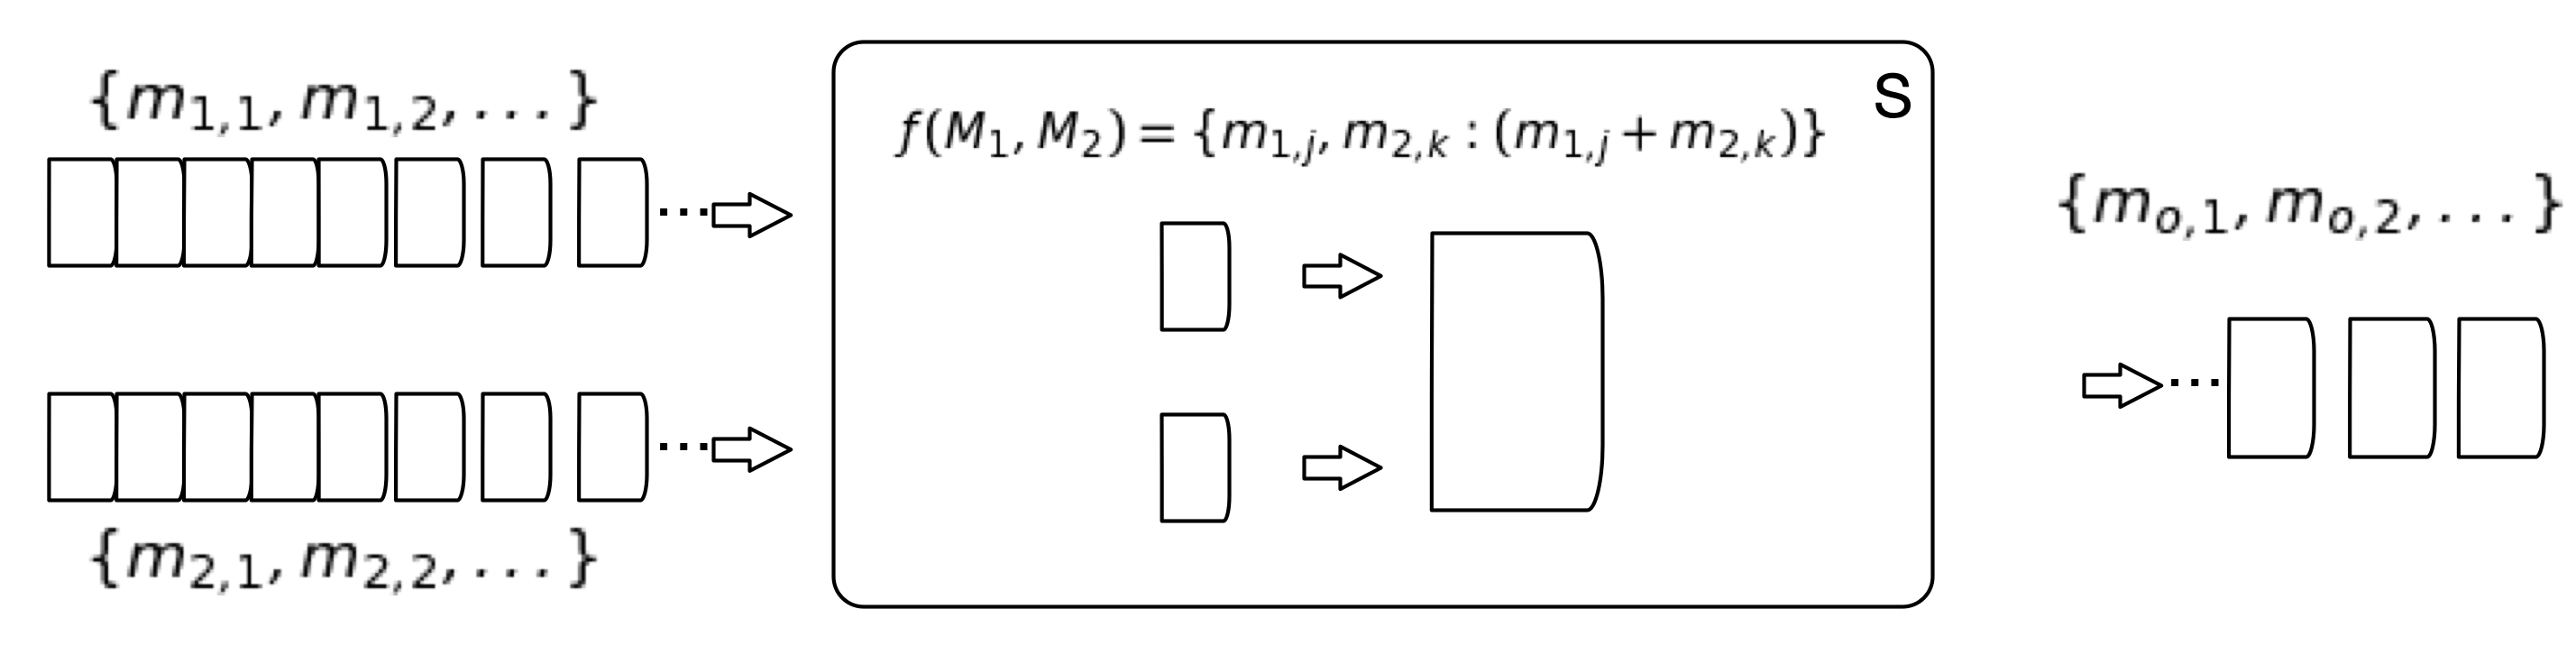
\includegraphics[scale=0.6]{stream_aggregator_function}
\centering
\caption {Service S integrates messages from multiple input streams $M_i$ to produce an aggregated output stream $M_o$ via $f$.}
\label{fig:stream_aggregator_function}
\end{figure}


\paragraph{Local State Aggregator Function} - Service $S$ observes an input stream $M_i$ which it integrates with a local (non-stream) queryable data store (see Figure \ref{fig:stream_local_state_aggregator_function}). Messages $m_i$ are integrated with query results $q_i$ to produce an output stream $M_i$. This type of service also requires management of state and scalability concerns similar to the Aggregator service, especially when the local data store is itself distributed. 

\begin{figure}[H]
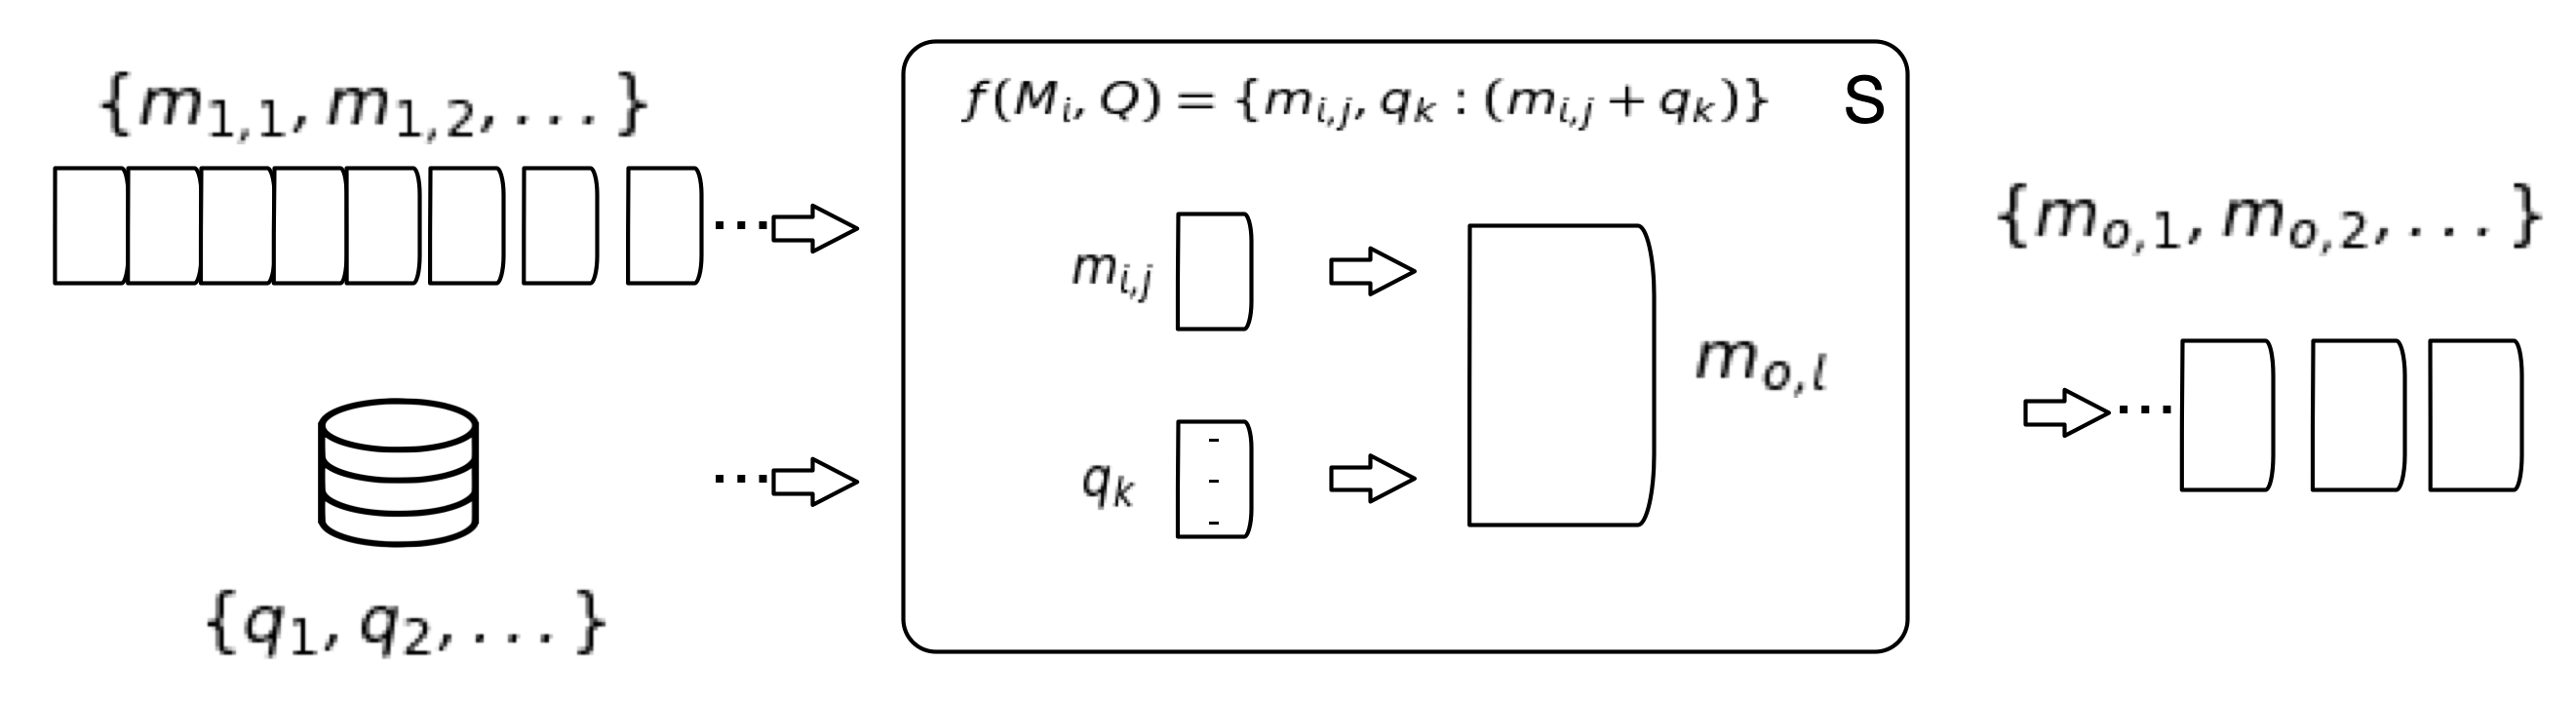
\includegraphics[scale=0.6]{stream_local_state_aggregator_function}
\centering
\caption {Service S aggregates $m_i$ with query results $q_i$ obtained from a local data store.}
\label{fig:stream_local_state_aggregator_function}
\end{figure}


\paragraph{Persistence Function} - Service $S$ observes messages $m_i$ and is responsible for persisting them to a data store where their contents can later be queried (see Figure \ref{fig:stream_persistence_function}). Although persistence of data to, and subsequent querying of data from, a store, such as a database, are comparatively more expensive operations than immediate reasoning over a live data stream, such mechanisms are necessary for situations where data may need to be accessed multiple times, or where data may need to be retained for audit purposes.

\begin{figure}[H]
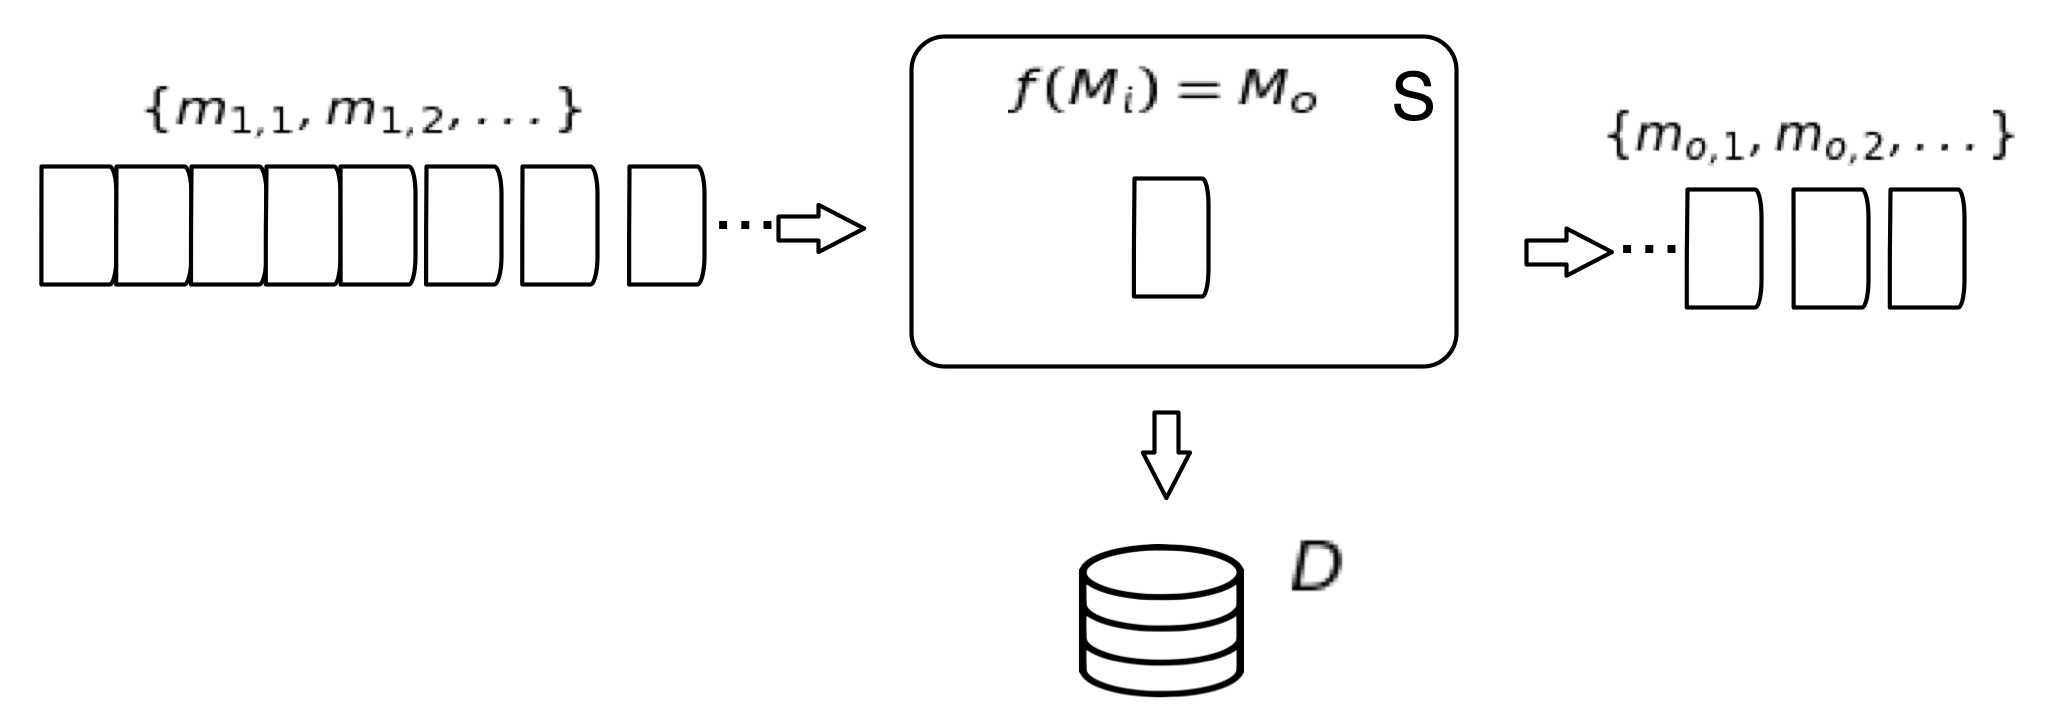
\includegraphics[scale=0.6]{stream_persistence_function}
\centering
\caption {Service $S$ processes messages $m_i$ into persistent storage. The output stream $M_o$ contains persistence confirmation and error events.}
\label{fig:stream_persistence_function}
\end{figure}

\paragraph{Query Function} - Service $S$ observes a stream of queries $Q_i$. The queries are fulfilled against a data store $D$ and the results emitted via the output stream $M_o$.

\begin{figure}[H]
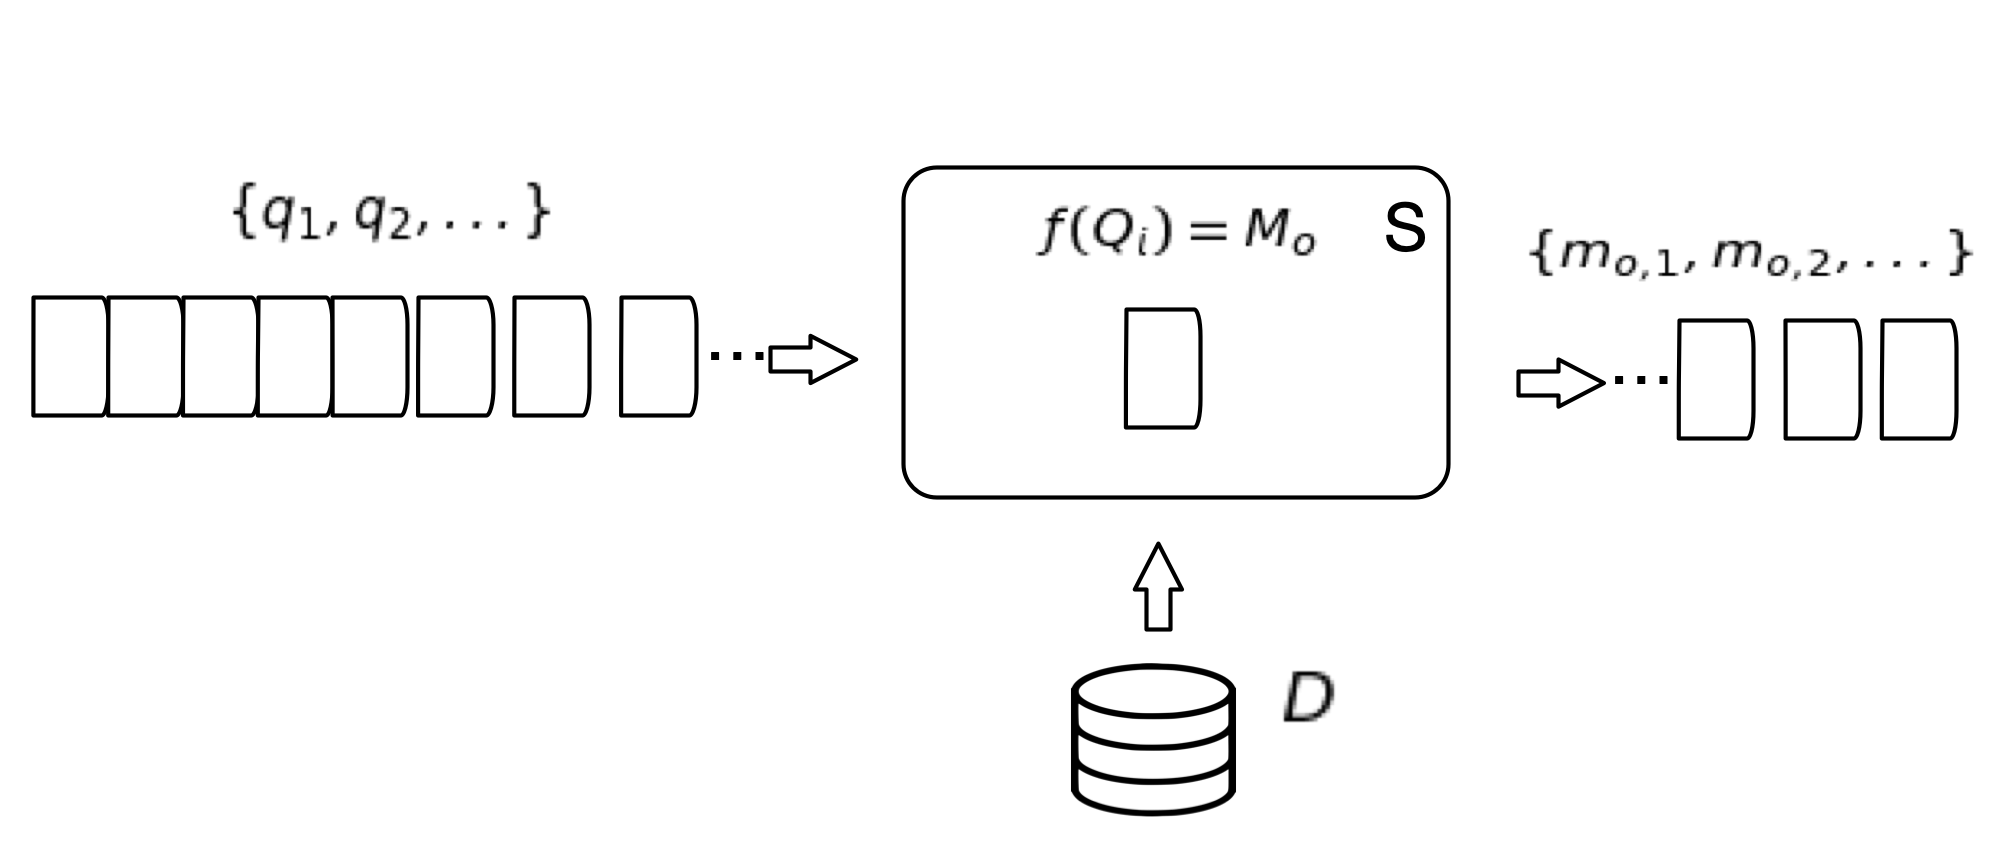
\includegraphics[scale=0.6]{stream_query_function}
\centering
\caption {Service S filters messages from input stream $M$ and only allows through those that pass the filtering condition.}
\label{fig:stream_query_function}
\end{figure}

The basic operations above can be combined to produce arbitrarily complex logic on data streams.

One of the key advantages of a service-oriented approach is that, because services are typically constantly executing, it naturally lends itself to an examination of the system's runtime characteristics. This applies to both service-internal characteristics that are related to each operation a service performs, as well as to external characteristics that relate to the contracts a service establishes with its dependencies. We consider both of these.

For each given operation $o_i \in S$ it is instrumental to understand the resource requirements of the operation on typical inputs and limiting factors that affect the efficiency with which the operation can be performed by $S$. Of particular interest are the per-operation profiles of:

\begin{itemize}
    \item CPU utilization
    \item RAM
    \item Secondary storage
    \item Network utilization
\end{itemize}

If $o_i$ is a long-running operation that takes multiple seconds to complete on average, a detailed distribution in time of each metric above may be necessary. If the operation can be completed at a sub-second rate then summary statistics (min, max, mean, median, inter-quartile range, 90th, and 99th percentiles) may be sufficient. This level of understanding is necessary in order to make sure that the service can adequately deal with the incoming message stream while the messages are first loaded into memory, since subsequent retrieval from secondary storage is several orders of magnitude slower and may cause further delays in processing. If $o_i$ is stateless, i.e. it does not require the storage and retrieval of any local state that depends on the content of each arriving message $m_j \in M_i$, then the service $S$ can be scaled "horizontally"\autocite{vaquero2011dynamically} with respect to $o_i$. Given that the performance-limiting condition of $o_i$ is known (CPU, memory, etc.), the ability of $S$ to efficiently deal with fluctuations in the rate of incoming messages $M_i$ can be successfully achieved simply by adding and removing servers that execute $S$ (see Figure \ref{fig:horizontal_vs_vertical_scaling}), which can be done automatically\autocite{mao2011auto}. If $o_i$ is stateful and requires access to databases, or predictable request routing via sessions, then horizontal scalability may not be possible and thus, detailed understanding of the performance profile and performance-limiting conditions of $o_i$ is even more important as vertical scaling of services is more expensive and challenging to accomplish, and may increase system complexity by necessitating data partitioning, for example\autocite{vaquero2011dynamically}.

\begin{figure}[H]
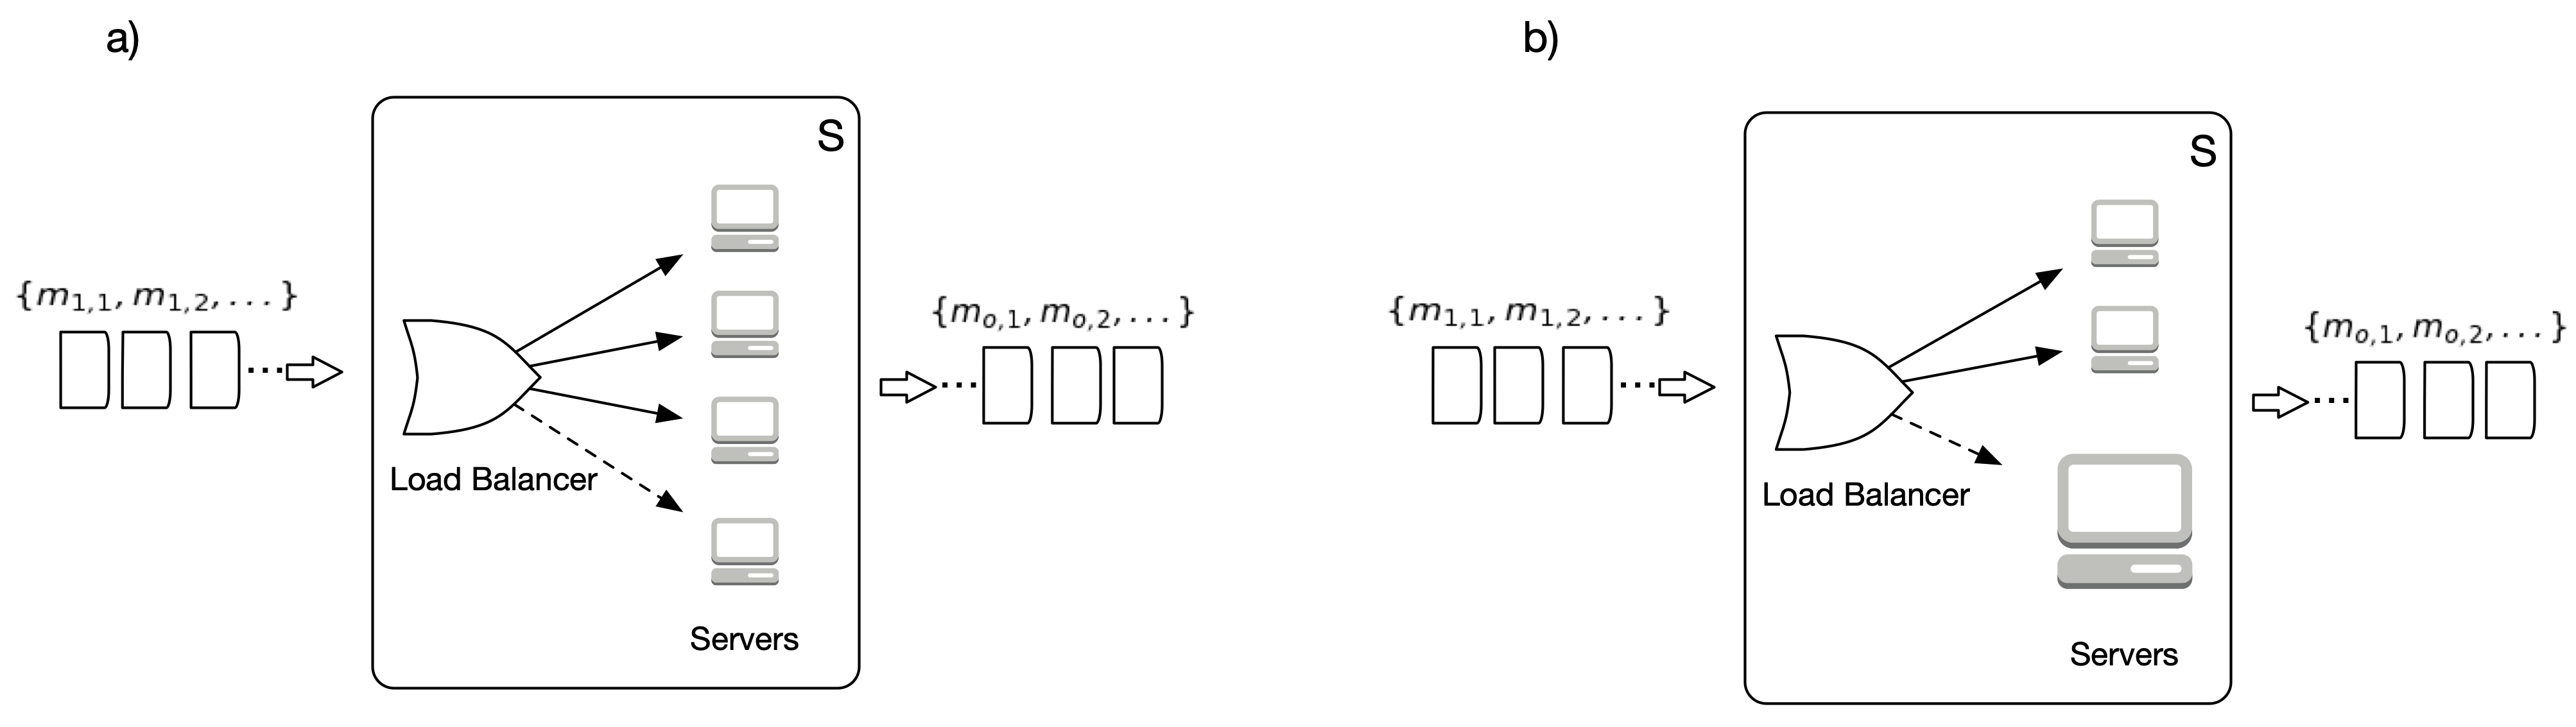
\includegraphics[scale=0.44]{horizontal_vs_vertical_scaling}
\centering
\caption {a) In horizontal scaling new servers are added and removed (dashed arrow) behind a load balancer as the rate of data stream $M_i$ fluctuates. b) In vertical scaling more powerful servers need to be launched (dashed arrow) to replace smaller servers (with potential service outage) when the rate of $M_i$ increases beyond capacity.}
\label{fig:horizontal_vs_vertical_scaling}
\end{figure}

Assume service $S$ implements operation $o$ supported by $n$ physical servers $V = \{v_j: j \in [1,n]\}$ by consuming a stream of incoming messages $M_i$. For a suitable time increment $t$, let $r_{M_i} = |M_i|/t$ be the incoming message arrival rate, and $r_{M_{o,j}} = |M_{o,j}|/t$ be the processing rate for server $v_j$. If $r_{M_i} > \sum_{j=1}^n r_{M_{o,j}}$, then $S$ will not be able to adequately process all of the incoming messages from $M_i$ and messages will either be lost or need to be backlogged while more servers are added to $S$ to deal with the incoming message rate. Since commissioning new servers takes considerable time and the timing and magnitude of increases in $r_{M_i}$ may be unpredictable, serious information loss may result if measures are not put in place to mitigate the message rate fluctuations. 

A queue is the mechanism that we put in place to address this concern (see Figure \ref{fig:queue}). A queue $Q$ is a message buffering system which consists of a set of $n$ "topics" $P = \{p_i: i \in [1,n]\}$, where each topic is a tuple of the form $p_i = (D_p,B_p,C_p)$. Here $D_p = \{d_i: i\in [1,k]\}$ is a set of $k$ data producers that put messages into $Q$, $B_p$ is a message buffer of max capacity $N_{max}$ dictated by underlying server hardware characteristics, containing a sequence of messages $\{m_t, m_{t-1},m_{t-2},....,m_1\}$ that are accessible in a Fist In First Out (FIFO) manner, and $C_p = \{c_i: i \in [1,l]\}$ is a set of $l$ consumers that are interested in observing messages from $p_i$.

\begin{figure}[H]
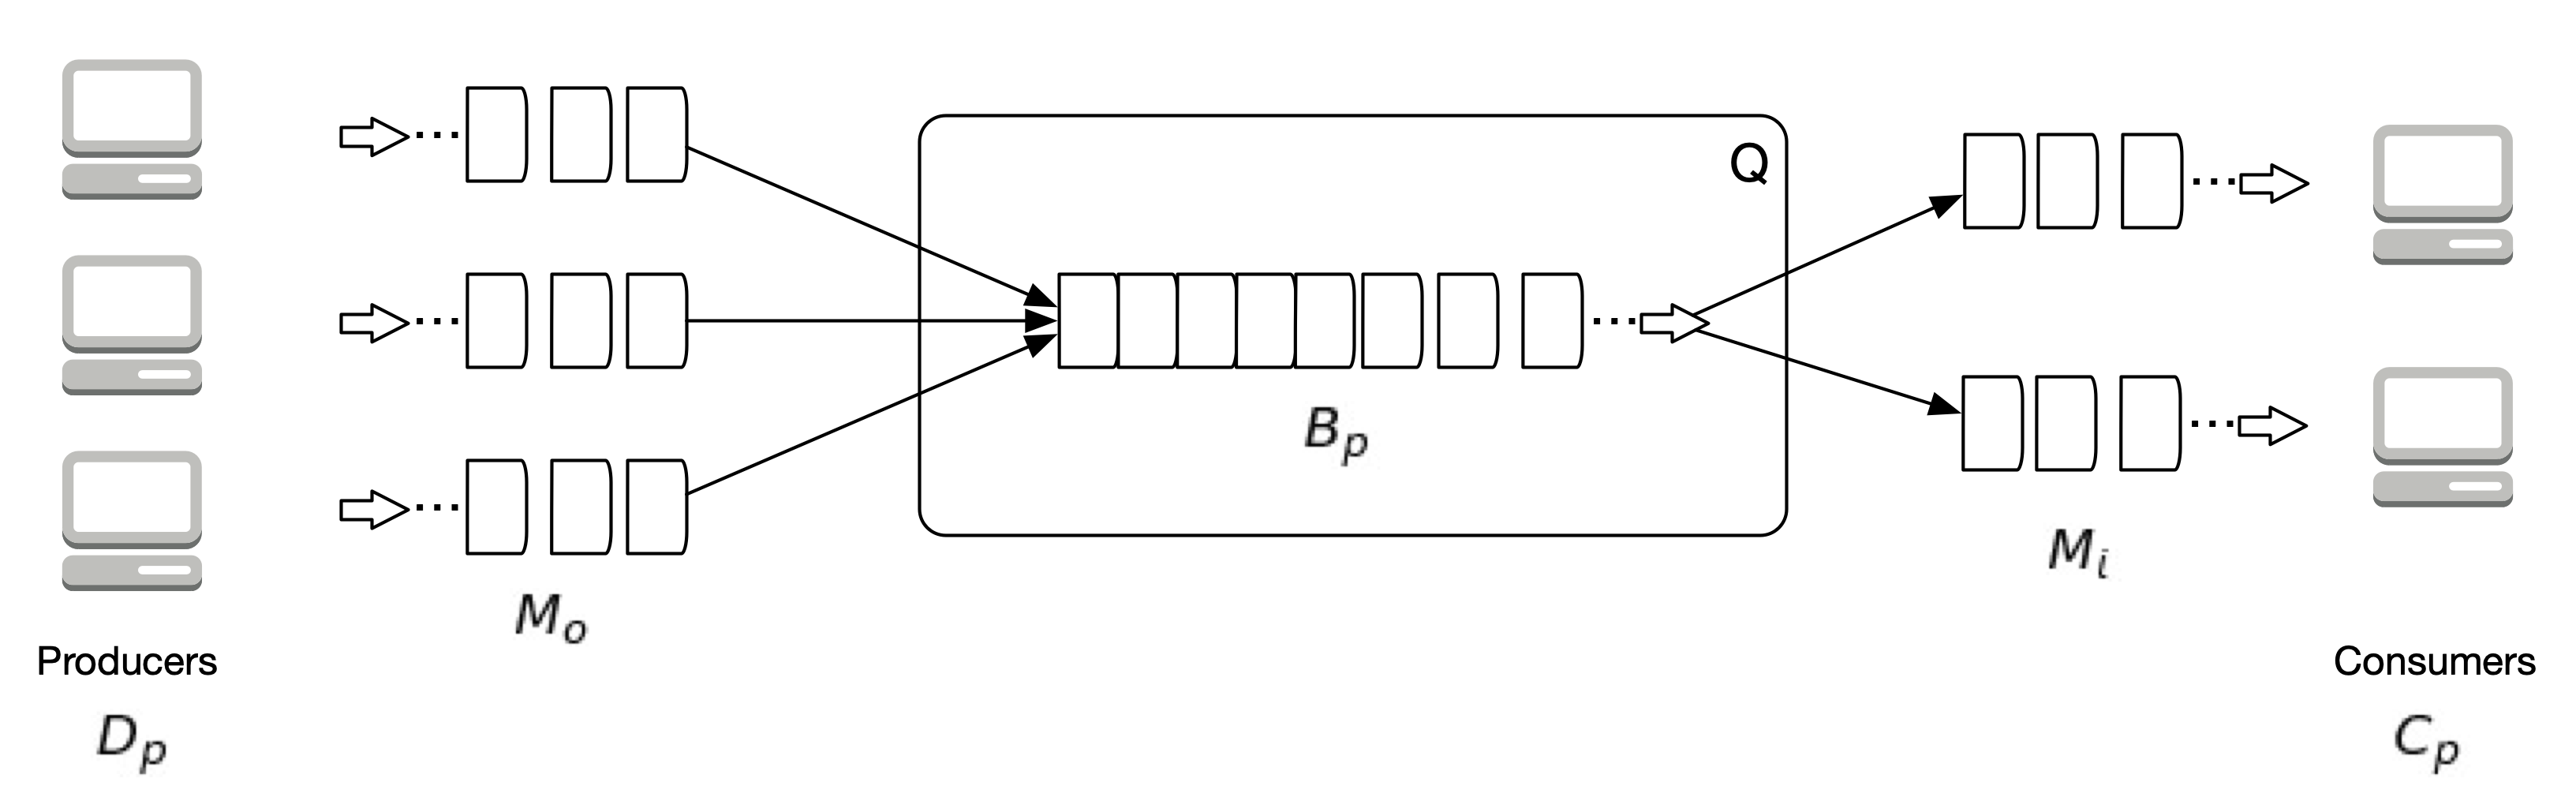
\includegraphics[scale=0.54]{queue}
\centering
\caption A queue $Q$ establishes a message buffer $B_p$ between a set of message producers $D_p$ and consumers $C_p$, for a given topic $p$.
\label{fig:queue}
\end{figure}

Messages arrive into a particular topic of $Q$ from all producers $D_p$, and are marked safe for deletion only when all of the subscribed consumers $C_p$ have observed a particular message. Thus, for topic $p_i$, the incoming message rate is $\displaystyle R_i = \sum_{j=1}^k r_{M_{o,j}}$ i.e. the sum of the message processing rates for all of the producers for this topic. The queue message processing rate $\displaystyle R_o = \min_{i \in [1,l]}\{r_{M_{o,i}}\}$ is the slowest message processing rate among all consumers. Assuming $R_i > R_o$ and that there are $N$ messages presently in $B_p$, there remains $t = \frac{N_{max} - N} {R_i - R_o}$ time before queue overflow occurs. The situation should then be remedied by allocating additional hardware to $Q$ or those services $S_i$ whose consumers are slowest, until the condition $R_o \ge R_i$ can be reliably maintained. If the queue does reach its maximum capacity overflow measures need to be put in place. Depending on the data stream in question data loss may or may not be acceptable. If data loss is acceptable then overflow messages can be simply discarded. If data loss is not acceptable then producers must block waiting for additional queue capacity to become available. This not only degrades performance locally, but can have a drastic effect on the entire system if the effects are allowed to percolate trough the complex distributed system. As message rates evolve through time with system load, the scheme above sets up a framework for flow control and hardware allocation within the architecture.

When designing a service-oriented system the interfaces of operations provided by the service are of utmost importance as they define the capabilities that the service offers to its clients. Of secondary, but also significant, importance is the set of Service-Level Agreements (SLAs)\autocite{wieder2011service} that a service advertises. These SLAs are a set of commitments that a service makes to its clients that describe the operational characteristics of the service, such as:

\begin{description}
    \item [Availability] - Guarantees related to the service uptime, maintenance outages, disaster recovery, etc.
    \item [Throughput] - The number of requests serviced per unit time.
    \item [Latency] - The delay between a request being sent and a response being received.
    \item [Abandonment Rate] - Proportion of requests that are never answered.
    \item [Error Rate] - Proportion of well-formed requests that result in an error.
\end{description}

Based on the SLAs that are advertised by a given service, the services that depend on it can make assumptions about expected runtime behavior, and take action when expectations are not met. Furthermore, when requirements evolve and features are added to or removed from a service, the impact on the advertised SLAs helps communicate the full effect of the changes. Lastly, the costs of operating a service are more clearly understood through the SLA framework, where improvements to a particular SLA metric, such as Transactions-Per-Minute (TPM) can be transparently traced to a corresponding increase in operational costs.

The set of services $\{S\}$ that communicate over data streams $\{M_{s,d}\}$, mediated by a set of queues $\{Q\}$ with a set of established SLAs $\{L_s\}$ together form the overall framework of Rheos that is used to tackle the challenges of large-scale genomic data processing in a manner the enables active tradeoffs between the competing constraints of cost, time, and accuracy. 

\section{Domain-specific Problems}

Having laid out the general data-streaming service-oriented architecture of Rheos in the previous section we now turn to a discussion of the set of actual domain-specific problems that need to be solved within the data-streaming paradigm in order to enable the comprehensive genomic characterization of large cohorts of samples within Rheos, as we have set out to do. We make use of the flow of data types from the most raw to the most refined (see Figure \ref{fig:ngs_flow}) to illustrate the challenges that need to be solved during transformation of the input data between each successive stage, first in summary form, and then in full detail, below.

\begin{figure}[H]
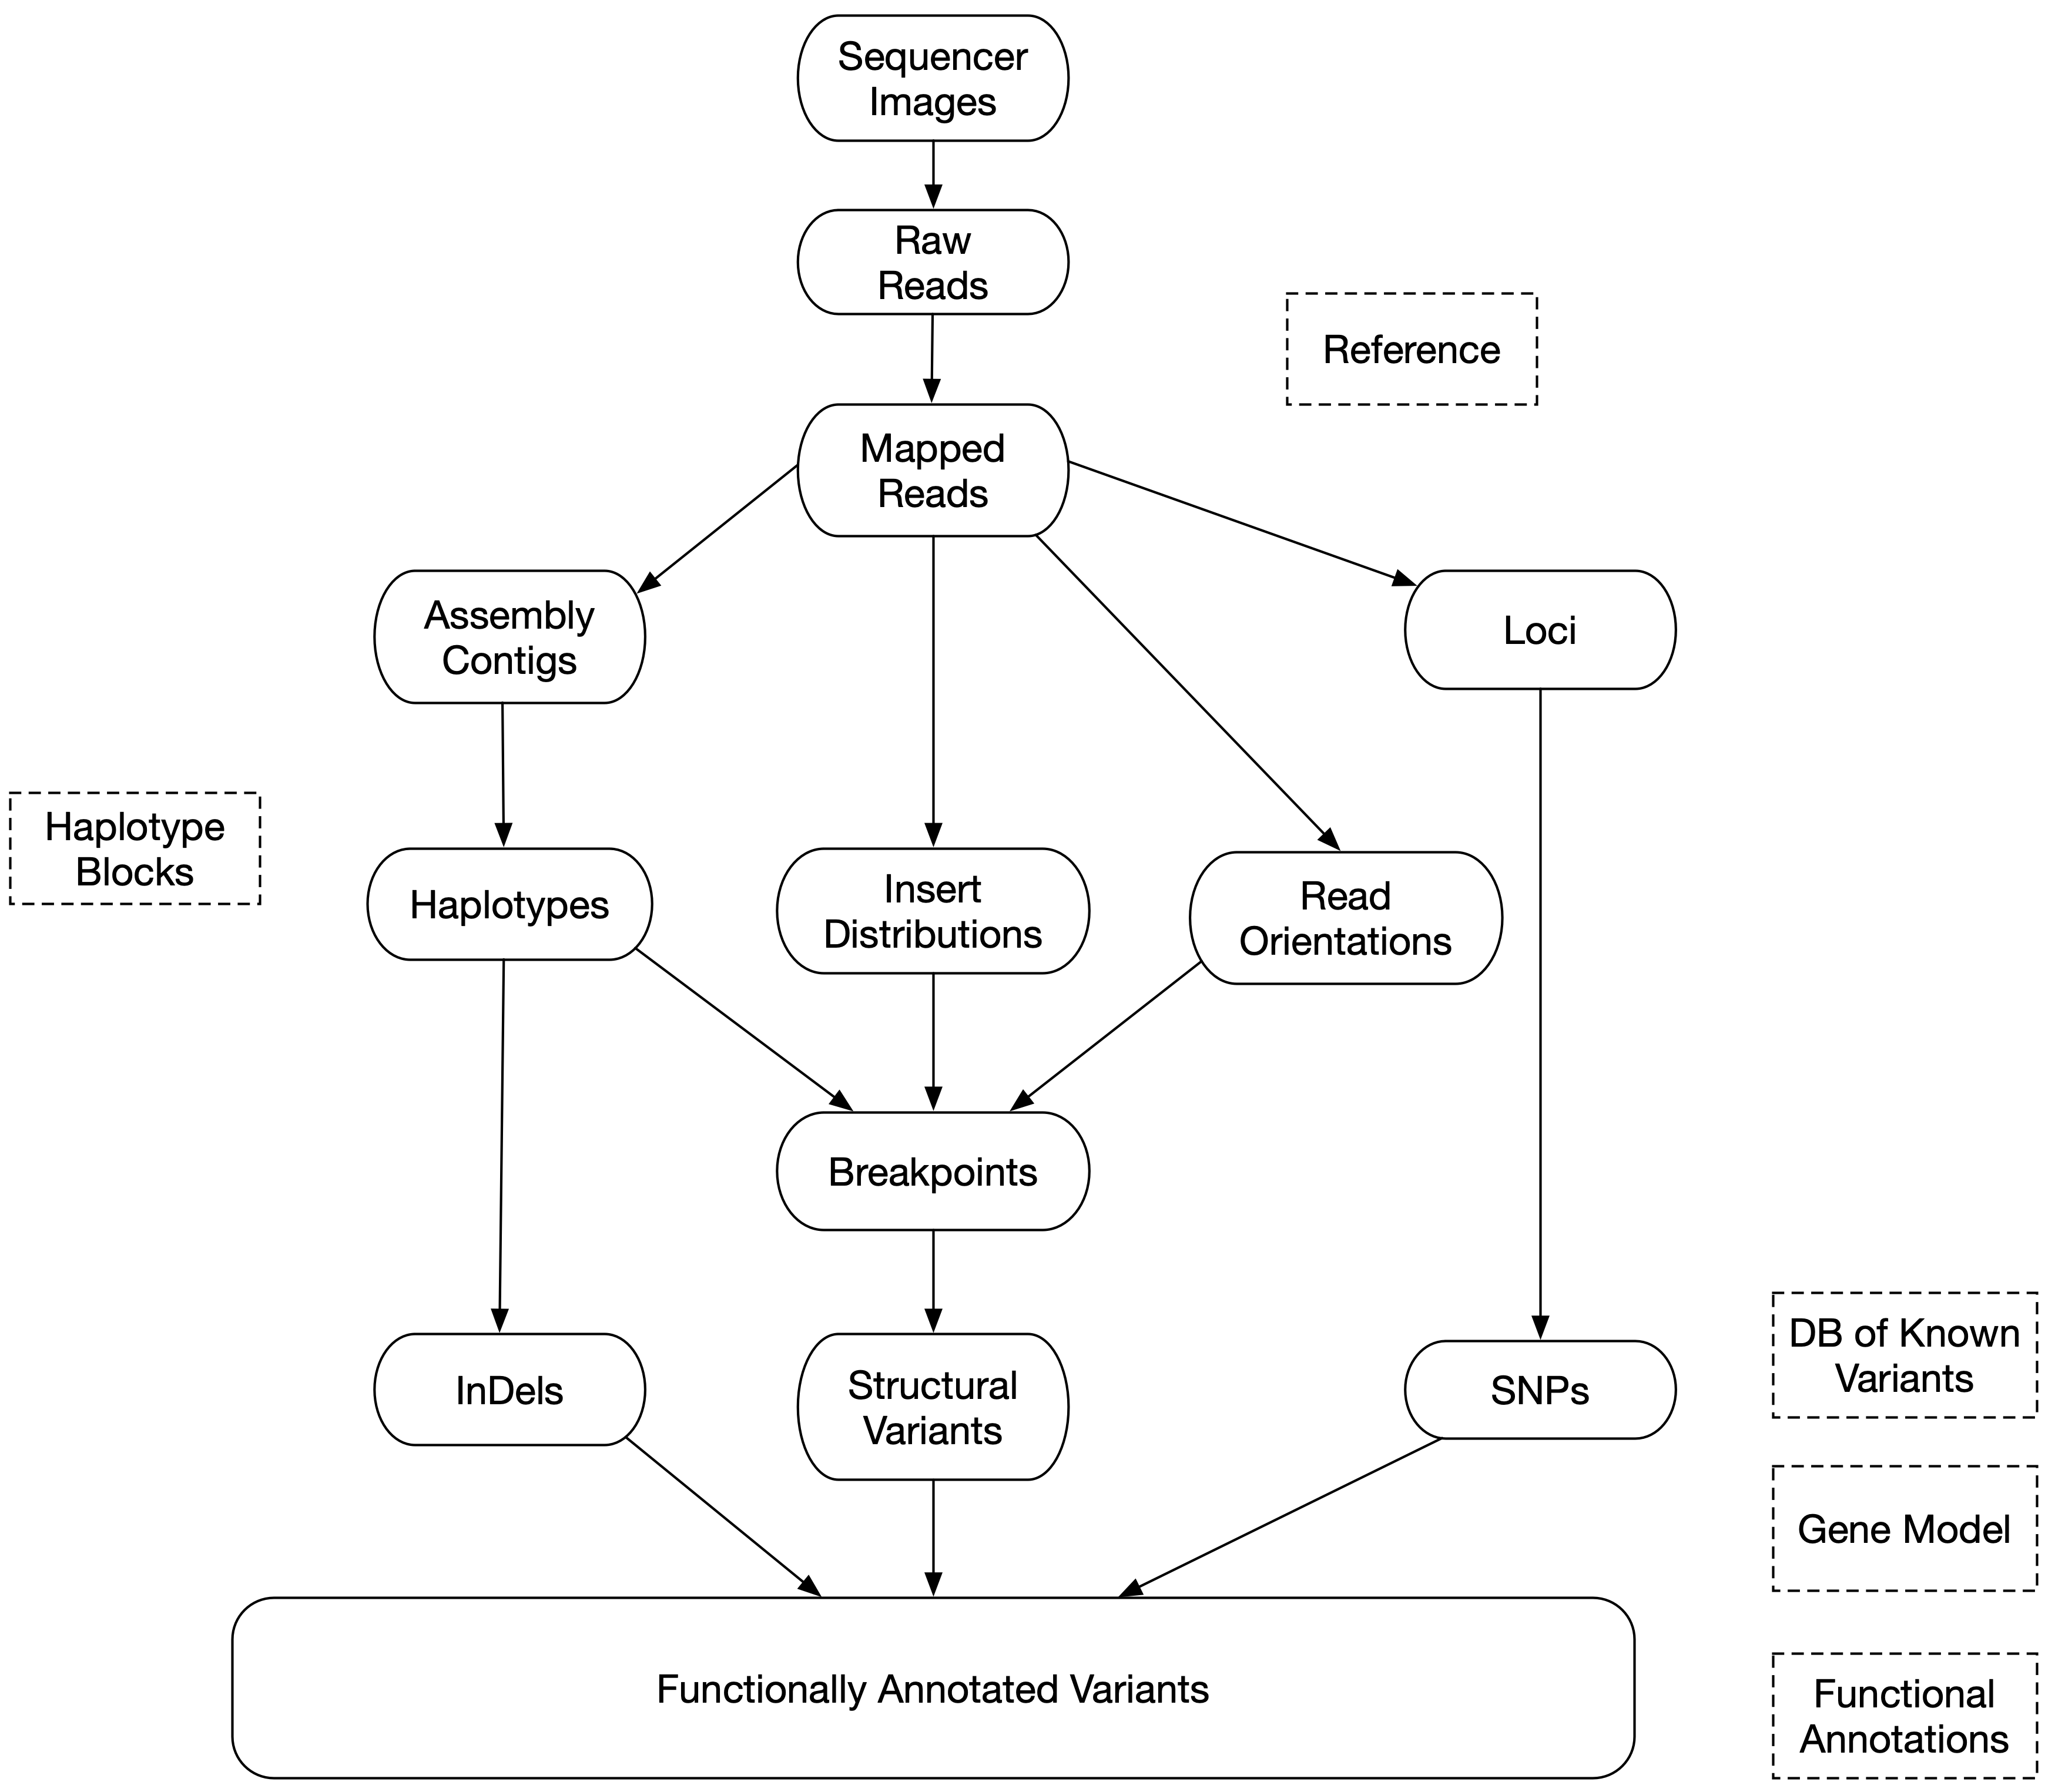
\includegraphics[scale=0.5]{ngs_flow}
\centering
\caption {The conceptual flow of data types within Rheos from the most raw - Sequencer Images, to the most refined - a set of Functionally Annotated Variants.}
\label{fig:ngs_flow}
\end{figure}
    
The most raw data type that is produced from a sequencing experiment is the set of raw image files generated by the sequencer. Although, conceptually, processing of the raw images could also be accomplished within Rheos, it is presently outside of the scope of this work. Instead, we assume the most basic data type to be raw sequencing reads, as found in a FASTQ\autocite{cock2009sanger} file. 





Describe specific problems that need to be addressed by the system in a stream-based formulation - how to go from a collection of raw reads to a set of annotated variants: map reads, perform QC filtering, model loci, assemble alternative haplotypes, call variants, filter variants, annotate, produce output.  


\begin{itemize}
    \item Perform read QC
    \item Align reads to reference
    \item Collect read stream statistics
    \item Assemble local read contigs
    \item Model individual loci
    \item Call variants (maybe need to split by variant types)
    \item Genotype variants
    \item Filter variants
    \item Annotate variants
    \item Output variants
\end{itemize}


\section{Services of Rheos}

Provide a mapping from the domain-specific problems onto a particular implementation in the data streaming architecture. List services, their responsibilities, contracts, etc.

\begin{description}
    \item [Metadata] - Take in metadata related to patients, samples, files, etc. In: Metdata records, Out: ingestion confirmation events.
    \item [Read Streaming] - Take data from outside the system (file, web service, etc) and turn it into a standard stream. In: files, external streams, Out: internal read stream.
    \item [Read Persistence] - Store reads on disk, index. In: read stream, Out: persistence confirmation events.
    \item [Read Statistics] - Look at read stream and calculate various approximate stats of interest - insert size, GC-bias,  etc. In: read stream, Out: running stats of interest
    \item [QC] - Compute QC score for reads. In: reads, Out: reads with QC score
    \item [Read Filtering] - Filter out low quality reads based on configured parameters. In: reads with QC score, Out: filtered reads.
    \item [Read Mapping] - Align reads to reference genome. In: stream of reads, Out: streams of mapped, unmapped, split reads.
    \item [Local Assembly] - Local assembly of reads into candidate haplotypes. In: stream of aligned reads, Out: Updated haplotypes event.
    \item [Haplotype Persistence] - Storage and lookup of candidate haplotypes. In: stream of reads, Out: persistence confirmation events, stream of haplotypes.
    \item [Variant Calling] - Evaluate candidate haplotypes for presence of variation. In: haplotype update events, Out: variant update events.
    \item [Variant Persistence] - Storage and lookup of variants. In: stream of reads, Out: persistence confirmation events, stream of variants.
    \item [Genotyping] - Genotype variant sites. In: variant update stream, Out: genotype update events.
    \item [Variant Filtering] - Filter out low quality variants. In: stream of variants, Out: filtered stream of variants.
    \item [Variant annotation] - Annotate variants for functional impact. In: stream of variants, Out: stream of annotated variants.
    \item [Output variants] - Format variants for external output. In: stream of variants, Out: files, external variant stream.
    \item [Notification] - Notify the user when events of interest occur. In: any stream, Out: stream of notifications.
\end{description}

\section{Proof of concept implementation}

Describe actual implementation efforts. Focus on very basic use case (take already mapped reads from a file, turn them into a stream, use stream to call SNPs, maybe some Indels/SVs). Demonstrate some comparison metrics compared to other callers. Demonstrate some service-level metrics (throughput etc.)

\section{Conclusions}
Rheos is great!